\section{Gasphasenabscheidungen}
\label{depositions}

Gasphasenabscheidungen sind ein Herstellungsverfahren für dünne Schichten, bei denen durch physikalische oder chemische Prozesse aus einer Gasphase eine dünne Schicht auf einer Oberfläche aufgewachsen wird.
Ihre drei Arten werden gemäß ihrer Funktionsweise als \textbf{Physikalische Gasphasenabscheidung} (PVD, Physical Vapor Deposition), \textbf{Chemische Gasphasenabscheidung} (CVD, Chemical Vapor Deposition) und \textbf{Atomlagenabscheidung} (ALD, Atomic Layer Deposition) bezeichnet, die im folgenden vorgestellt werden.

Ihnen ist allgemein, dass einzelne Atome oder Moleküle aus der Gasphase auf der Oberfläche auftreffen, dort physikalisch oder chemisch adsorbiert werden und so mit vorhersehbarer Rate eine dünne Schicht eines gewünschten Materiales bilden.
Dennoch hat jeder Prozess seine eigenen Eigenschaften, die es ihm ermöglichen, verschiedene Materialarten mit unterschiedlicher Genauigkeit aufzuwachsen.
Tabellen \ref{tab:deposition-comparison} und \ref{tab:deposition-materials} sollen einen kurzen Überblick darüber verschaffen, bevor die Prozesse im einzelnen vorgestellt werden.
Alle Prozesse finden in speziellen Abscheidungskammern oder Reaktoren statt, über die Abbildung \ref{fig:reactors} einen kurzen Überblick geben soll.

\begin{figure}
  \captionsetup[subfigure]{format=plain}
  \def\chamberwidth{0.3\textwidth}
  \def\subcaptionwidth{0.65\textwidth}

  \parbox[c]{\chamberwidth}{
    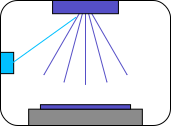
\includegraphics[width=\linewidth]{reactors-a}
  }\hfill
  \parbox[c]{\subcaptionwidth}{
    \subcaption{Sputter-Kammer (PVD):
      Ein Elektronenstrahl (links) schlägt Atome aus dem Target (oben), die sich auf dem Substrat (unten) als dünne Schicht absetzen
    }
    \label{fig:depochamber-a}
  }

  \vspace{1em}

  \parbox[c]{\chamberwidth}{
    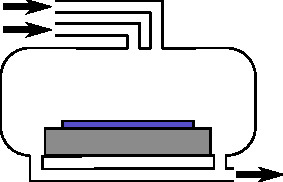
\includegraphics[width=\linewidth]{reactors-b}
  }\hfill
  \parbox[c]{\subcaptionwidth}{
    \subcaption{Injektions-Kammer (CVD, ALD):
      Precursorgase strömen von oben über das Substrat, wo sie durch chemische Reaktionen dünne Schichten bilden.
      Nebenprodukte der Oberflächenreaktionen werden nach unten aus dem Reaktor gespült
    }
    \label{fig:depochamber-b}
  }

  \vspace{1em}

  \parbox[c]{\chamberwidth}{
    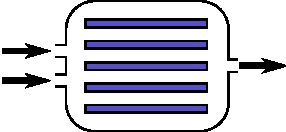
\includegraphics[width=\linewidth]{reactors-c}
  }\hfill
  \parbox[c]{\subcaptionwidth}{
    \subcaption{Batch-Reaktor (CVD, ALD):
      Gase strömen zwischen Stapeln von Substraten, auf deren Oberfläche durch chemische Reaktionen dünne Schichten abgeschieden werden.
      Nebenprodukte werden mit dem Gasstrom aus dem Reaktor gespült
    }
    \label{fig:depochamber-c}
  }

  \caption[Abscheidungskammern und -reaktoren]{Abscheidungskammern und -reaktoren}
  \label{fig:reactors}
\end{figure}

\begin{table}
  \oddrowcolors
  \caption[Prozesscharakteristiken der Abscheidungsarten]{Vergleich der Abscheidungsarten}
  \label{tab:deposition-comparison}
  \begin{tabularx}{\textwidth}{|Xccc|}
    \hline
    \textbf{Eigenschaften} & \textbf{PVD}    & \textbf{CVD}       & \textbf{ALD}         \\
    \hline
    reaktiv                &                 & \cmark             & \cmark               \\
    kontinuierlich         & \cmark          & \cmark             & zyklisch             \\
    Gas-Edukte             & Atome, Moleküle & Precursor-Moleküle & Precursor-Moleküle   \\
    \# Edukte              & 1               & 1+                 & 2+                   \\
    Nebenprodukte          &                 & \cmark             & \cmark               \\
    Wachstumsrate          & $\sim t$        & $\sim t$           & $\sim n_\text{cyc.}$ \\
    \hline
  \end{tabularx}
\end{table}

\begin{table}
  \centering
  \begin{tabularx}{\textwidth}{XXXXXXXXX}
    ~            & \angled{Metalle} & \angled{Legierungen} & \angled{Metalloxide} & \angled{Nitride} & \angled{Chloride} & \angled{Silizium} & \angled{Siliziumoxid} & \angled{Diamant} \\
    \hline
    \textbf{PVD} & \cmark           & \cmark               & ~                    & ~                & ~                 & \cmark            & ~                     & ?                \\
    \textbf{CVD} & \cmark           & ?                    & \cmark               & \cmark           & \cmark            & \cmark            & \cmark                & ?                \\
    \textbf{ALD} & \cmark           & ?                    & \cmark               & \cmark           & \cmark            & \cmark            & \cmark                & \cmark           \\
  \end{tabularx}
  \caption[Mögliche Produkte der Abscheidungsarten]{Mögliche Produkte der Abscheidungsarten.
    Weitergehende Informationen finden sich in der Literatur für PVD\todo[inline]{cite}, CVD\todo[inline]{cite} und ALD\cite{puurunen_surface_2005}.
  }
  \todo[inline]{Referenzen für abgeschiedene Systeme}
  \label{tab:deposition-materials}
\end{table}

\subsection{Physikalische Gasphasenabscheidung}

Physikalische Gasphasenabscheidungen (PVD, Physical Vapor Deposition) sind eine grundlegenden Abscheidungsart, die nichtreaktiv mit einzelnen Atomen funktioniert.
Zu ihnen zählt beispielsweise Sputtering, bei dem aus einem Block des gewünschten Materiales (Target) per \todo{wirklich Elektronen?}Elektronen- oder Ionenstrahl kontinuierlich Atome herausgeschlagen werden, die sich dann auf dem Substrat absetzen und dort zu einer dünnen Schicht verbinden.
Anhand der Energien der herausschlagenden Partikel und deren \todo{Größe des?}Teilchenstrom lässt sich dabei die Wachstumsrate und Qualität des abgeschiedenen Dünnfilmes beeinflussen.
Durch den statistischen Charakter der Abscheidungsorte resultiert Sputtering in Abhängigkeit des abgeschiedenen Materiales und der Umgebungsbedingungen meist in glatten Filmen\cite{svorcik_annealing_2011}, bei denen prozessbedingt keine Kontrolle der Schichtdicke im Sub-Nanometer-Bereich möglich ist.
Gemischte Systeme wie Legierungen und mehrlagige Schichten werden durch Nutzung mehrerer Targets ermöglicht\cite{cammarata_nanoindentation_1990}.

\subsection{Chemische Gasphasenabscheidung}

Während einer Chemischen Gasphasenabscheidung (CVD, Chemical Vapor Deposition) adsorbieren sogenannte Precursormoleküle physikalisch auf dem Substrat und reagieren im Anschluss mit an der Oberfläche befindlichen Atomen.
Dabei werden entweder Teile des Precursors auf der Oberfläche hinterlassen oder von vorherigen Reaktionen verbliebene Precursorliganden von der Oberfläche entfernt, wodurch bei entsprechender Prozessgestaltung gewünschte Stöchiometrien und Bindungen bevorzugt gebildet werden.
Abbildung \ref{fig:ald-schema} stellt diese Vorgehensweise für ALD-Prozesse dar, die eine Spezialisierung von CVD-Prozessen sind und im nächsten Abschnitt vorgestellt werden.
Da es sich um einen kontinuierlichen Prozess handelt, befinden sich meist zwei Precursorgase gleichzeitig im Reaktor, wo sie idealerweise erst auf der Oberfläche miteinander reagieren, da Reaktionen zwischen ihnen in der Gasphase neben einem erhöhtem Gasverbrauch zu Verunreinigungen und Unebenheiten führen können.

Für erfolgreiche Abscheidungsprozesse ist es wichtig, neben passenden Umgebungsbedingungen auch Precursormoleküle zu wählen, die einerseits eine hohe Qualität des Filmes gewährleisten, andererseits kompakt genug sind, um hohe Wachstumsraten zu ermöglichen.
Zudem sollten die gasförmigen Nebenprodukte inert sein, um nicht mit der Oberfläche oder der Reaktorwand zu reagieren, während sie mit dem kontinuierlichen Gasfluss aus dem Reaktor gespült werden.
Auch eine physikalische Adsorption der Nebenprodukte auf der Oberfläche kann den Dünnfilm verunreinigen.
Dabei sind stets die Prozesstemperaturen, -drücke, Reaktionsbarrieren und die Stabilität aller involvierten Moleküle zu betrachten, wodurch Chemische Gasphasenabscheidungen oft monatelanger Arbeit justiert werden müssen.
Wie bei PVD lässt sich die Schichtdicke auf mehrere Nanometer genau kontrollieren, was hinsichtlich einer gegenüber ALD vergleichsweise hohen \todo{ref}Wachstumsrate für viele Anwendungen ausreichend ist.

\todo[inline]{Beispiel Precursor-Moleküle}
\missingfigure{Beispiel Precursor-Moleküle}

\subsection{Atomlagenabscheidung}

\begin{figure}
  \centering
  \def\svgwidth{\textwidth}
  \input{img/ald-schema.pdf_tex}
  \caption[ALD-Schema]{ALD-Schema: asd ald}
  \label{fig:ald-schema}
\end{figure}

Als Variation einer Chemischen Gasphasenabscheidung entstanden Atomlagenabscheidungen (ALD, Atomic Layer Deposition) mit dem Ziel\todo{Referenz}, konforme dünne Schichten kontrolliert in einzelnen Atomlagen mit Sub-Nanometer-Genauigkeit der Schichtdicke aufwachsen zu lassen.
Dazu werden zwei Precursorgase wechselweise in separaten Schritten (Halbzyklen) in den Reaktor geleitet, wo sie wie bei CVD-Prozessen mit der Oberfläche reagieren und so langsam eine Schicht aufwachsen (Abbildung \ref{fig:ald-schema}).
Zwischen den Precursorschritten entfernen Spülschritte mit inertem Gas verbleibende Precursormoleküle und Nebenprodukte aus dem Reaktor und verhindern so gleichzeitige Reaktionen beider Precursorgase.
So werden einerseits Gasphasenreaktionen vermieden, andererseits limitiert die Sättigung der Oberfläche mit Precursorliganden in jedem Precursorschritt die Zunahme der Dicke pro Zyklus.
Die Wachstumsrate aus den kontinuierlichen Prozessen wird somit von dem Growth-per-Cycle-Wert (GPC) abgelöst, der angibt, wie viel eine Schicht im Schnitt pro Zyklus wächst.
Über die Zahl der Zyklen lässt sich somit die Dicke der gewachsenen Schicht genauer als mit kontinuierlichen Abscheidungen steuern, was sich aber in langsameren Abscheidungsprozessen äußert.

Anders als der Name des Prozesses vermuten lässt, werden aufgrund sterischer Hinderung (Abbildung \ref{fig:sterichindrance}) der Precursorliganden keine kompletten Atomlagen in jedem Zyklus aufgebracht.
Üblicherweise erreichen ALD-Prozesse maximal zu \todo{referenz}\SI{35}{\percent} einer Monolage, doch sorgen die teils recht großen Precursormoleküle mit größerem Radius der sterischen Hinderung für geringere GPC-Werte.
Die Suche nach möglichen Precursorpaaren und Prozessparametern unterliegt ansonsten gleichen Anforderungen wie bei CVD.
Eine ausführlichere Übersicht zu Atomlagenabscheidungen und zu möglichen Precursorpaaren für verschiedene Materialien findet sich in Referenz \cite{puurunen_surface_2005}.

\begin{figure}
  \centering
  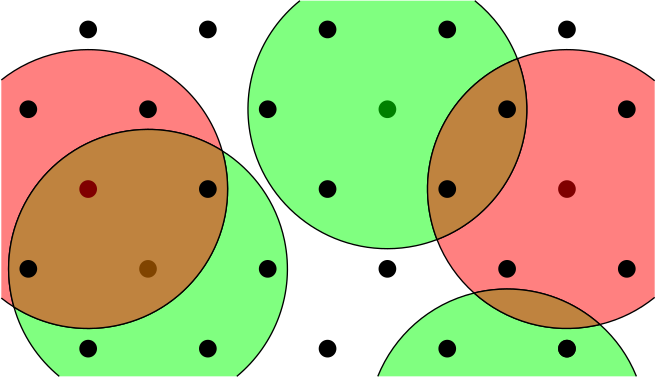
\includegraphics[width=0.5\textwidth]{sterichindrance_noalpha}
  \caption[Sterische Hinderung]{Sterische Hinderung auf einem Gitter:
    Angelagerte Precursor-Liganden verhindern Reaktionen auf benachbarten Gitterpunkten.
    Überlagerungsfreie Positionen in größerem Abstand akzeptieren weiterhin Precursor-Reaktionen.
  }
  \label{fig:sterichindrance}
\end{figure}

\subsection{Simulation von Gasphasenabscheidungen}

\begin{table}
  \oddrowcolors
  \caption[Überblick über Methoden zur Simulation von Gasphasenabscheidungen]{Überblick über Methoden zur Simulation von Gasphasenabscheidungen}
  \label{tab:deposition-simulations}
  \todo[inline]{Referenzen!}
  \begin{tabularx}{\textwidth}{|XXlX|}
    \hline
    Methode                           & Anwendungsfeld                       & Größenordnung     & Grundlagen                          \\
    \hline
    Finite Elemente Methode (FEM)     & Gasfluss und -verbrauch in Reaktoren & makroskopisch     & Navier-Stokes-Gl., Reaktionskinetik \\
    Kinetic Monte Carlo (KMC)         & Wachstums\-simulationen              & mikroskopisch     & Reaktionsraten, Gitternäherungen    \\
    Molekular\-dynamik (MD)           & Material\-unter\-suchungen           & < 1.000.000 Atome & klassische Interaktionspotentiale   \\
    Dichte\-funktional\-theorie (DFT) & Reaktionspfade                       & < 1.000 Atome     & Elektronendichten                   \\
    \hline
  \end{tabularx}
\end{table}

\todo[inline]{fig:methodscales}
\missingfigure{fig:methodscales}

Für die Simulation von Gasphasenabscheidungen stehen verschiedene numerische Methoden zur Verfügung, die die Darstellung auf unterschiedlichen Zeit- und Größenordnungen ermöglichen (Tabelle \ref{tab:deposition-simulations})\todo{fig:methodscales}.
Jede dieser Methoden basiert auf anderen Annahmen und Formulierungen, so dass sich ihre Anwendungsgebiete zwar nur marginal überschneiden, aber der Transfer von Ergebnissen zwischen den Methoden zu präziseren Vorhersagen führen kann.
So können FEM-Reaktorsimulationen den Gasverbrauch an charakteristischen Punkten der Oberfläche durch KMC-Simulationen ermitteln, welche wiederum auf DFT-Daten für Reaktionsraten und -energien zurück greift.
Bisherige Simulationen verzichten meist auf ein strukturelle Betrachtungen der abgeschiedenen Schicht, wie sie etwa mit molekulardynamischen Rechnungen möglich werden, obwohl sie besonders in der Nanoelektronik von Interesse werden.
